% ----------- Document settings -----------
\documentclass[nonacm,sigconf]{acmart}
% ====================================================
% General layout, typography & document-wide settings
% ====================================================

% ----------- Document settings -----------
\def\documentTitle      {Onderzoeken schrijven in Latex} % replace with actual document title
\def\documentSubtitle   {Een basis bestand voor een gelijke uitstraling} % replace with actual subtitle if any, else leave empty
\def\authorName         {John Doe} % replace with actual author name
\def\authorEmail        {JohnDoe@gmail.com} % replace with actual author email
\def\institutionName    {Harvard} % replace with actual institution name
\def\institutionCountry {Verenigde Staten} % replace with actual institution location
\def\institutionCity    {Massachusetts} % replace with actual institution location
\def\dueDate            {Oktober 2025} % replace with actual due date

\def\editorsVersion     {false} % true om editorsnote e.d. te tonen, false voor verbergen
\def\makeTitlePage      {true}  % true om titelpagina te maken, false om over te slaan
\def\makeTOCpage        {true}  % true om inhoudsopgave te maken, false om over te slaan

\def\listMark           {-} % itemize marker, e.g. '-', '*', '\textbullet', etc.

%----------- DONT TOUCH BELOW THIS LINE -----------
\usepackage{xparse}
\usepackage{xstring}

% ----------- Encoding & Fonts -----------
\usepackage[T1]{fontenc}
\usepackage[utf8]{inputenc}
\usepackage{scalefnt}

% ----------- Page layout -----------
\usepackage{expl3}
\usepackage{array}
\setlength{\columnsep}{0.333in}
\renewcommand{\baselinestretch}{1.05}
\setlength\parindent{2mm}
\setlength{\footskip}{40pt} %set footer size bigger to avoid overlap with text
\usepackage{geometry}
\geometry{
    a4paper,
    left=15mm,
    right=15mm,
    top=15mm,
    bottom=15mm,
}

% ----------- Table of Contents -----------
\usepackage{titletoc}
\setcounter{tocdepth}{2} % include subsections in TOC
%
 \titlecontents{section}
 [0] % i
 {\vspace{0.05cm}}
 {\thecontentslabel\enspace}%\thecontentslabel
 {}
 {\titlerule*[0.1cm]{.}\contentspage}%]

 \titlecontents{subsection}
 [1em] %
 {\vspace{0.05cm}}
 {\thecontentslabel\enspace}%\thecontentslabel
 {\hspace*{1em}}
 {\titlerule*[0.1cm]{.}\contentspage}


% ----------- Typography -----------
\usepackage{microtype} % subtle spacing & justification improvements

% ----------- Headings -----------
\usepackage{titlesec}
\titleformat{\section}{\large\bfseries}{\thesection}{1em}{}
\titleformat{\subsection}{\normalsize\bfseries}{\thesubsection}{0.75em}{}

% ----------- Lists -----------
\usepackage{enumitem}
\setlist[itemize]{
    leftmargin = *,
    listparindent = 10mm,
    label = {\listMark} % makes the default item marker a dash
}

% ----------- Figures & Tables -----------
\usepackage{graphicx}
\usepackage{subcaption}
\usepackage{tcolorbox}
\usepackage{float}
\usepackage{tabularx}
\usepackage{booktabs} % professional tables
\usepackage[table]{xcolor}
\usepackage{environ}

% Caption formatting
\usepackage{caption}
\captionsetup[table]{
    name=Tabel,                  % rename "Table" to "Tabel"
    labelfont={bf},              % "Tabel 1:" in bold
    textfont={normalfont},       % caption text in normal (non-bold)
    labelsep=colon               % ensures "Tabel 1:" (with colon)
}

\captionsetup[figure]{
    name=Figuur,                 % rename "Figure" to "Figuur"
    labelfont={bf},              % "Figuur 1:" in bold
    textfont={normalfont},       % caption text in normal (non-bold)
    labelsep=colon               % ensures "Figuur 1:" (with colon)
}

% ----------- Footnotes -----------
\usepackage[hang,flushmargin]{footmisc}

% ----------- Hyperlinks -----------
\usepackage[
    colorlinks=true,
    linkcolor=blue,
    citecolor=blue,
    urlcolor=blue,
]{hyperref}

% ----------- Column balance -----------
\usepackage{balance}

% ----------- Bibliography -----------
\usepackage[backend=biber,style=apa]{biblatex}
\DeclareLanguageMapping{dutch}{dutch-apa}
\DefineBibliographyStrings{dutch}{andothers = {et al.}}
\addbibresource{main.bib}
\setlength\bibitemsep{0.25em}

% ----------- ACM-style tweaks (optional) -----------
\settopmatter{printacmref=false}
\setcopyright{none}
\settopmatter{printfolios=true}
\renewcommand\footnotetextcopyrightpermission[1]{}

% ----------- Editors/general version -----------
\usepackage{comment}
\usepackage{ifthen}
\newboolean{editorsversion}
\setboolean{editorsversion}{\editorsVersion}  % change to false for student version


% ----------- Paper layout information -----------
\title{\documentTitle}
\subtitle{\documentSubtitle}

\author{\authorName}
\date{\dueDate}
\email{\authorEmail}
\affiliation{
    \institution{\institutionName}
    \city{\institutionCity}
    \country{\institutionCountry}
}

\hypersetup{
    pdfauthor={\authorName},
    pdftitle={\documentTitle},
    pdfborder={0 0 0}
}

% When \begin{document} is written, also add \maketitle and \tableofcontents there. (if settings are true)
\AtBeginDocument
{%
    \ifthenelse{\equal{\makeTitlePage}{true}}{%
        \maketitle
    }{}
    \ifthenelse{\equal{\makeTOCpage}{true}}{%
        \tableofcontents
        \newpage
    }{}
}% % import custom general paper settings
% --------------------------------
% This file contains a custom set
% of commands to make writing
% LaTeX easier
% --------------------------------

% makes 0.05 inches of horizontal space
\newcommand{\vertspace}{\vspace{0.05in}}

% writes centered italic text 80% width of the page/column and gives top & bottom padding
\newcommand{\question}[1]{\vertspace\begin{center}\parbox{0.8\linewidth}{\centering\textit{#1}}\end{center}\vertspace}

% Writes a single paragraph of Lorum Ipsum text
\newcommand{\lorem}{Lorem ipsum dolor sit amet, consectetur adipiscing elit. Nullam eget tortor a urna ornare pellentesque. Integer sit amet purus nec sem iaculis euismod. Duis at ipsum eu libero pharetra egestas. Quisque eleifend odio velit, at sollicitudin metus dictum eu. Integer nec mi congue, gravida nibh sed, faucibus mauris. Sed vel ipsum lobortis felis gravida dignissim. Curabitur vestibulum turpis eu orci lacinia consectetur.}

% APA style qoutes
\usepackage{xstring}
\newcommand{\qoute}[3]{%
  % Count the number of words in the quote
  \StrCount{#1}{ }[\woordenaantal]%
  \ifthenelse{\woordenaantal < 39}{``\textit{#1}'' (\citeauthor{#2}, \citeyear{#2}, p. #3)}% Kort citaat (minder dan 40 woorden)
  {
    \vertspace
    \begin{flushright}
      \parbox{0.95\linewidth}{\textit{#1}}
      (\citeauthor{#2}, \citeyear{#2}, p. #3)
    \end{flushright}
    \vertspace % Lang citaat (40 woorden of meer)
  }
}

% cites like \parencite[prenote][postnote]{cite}
\newcommand{\parencite}[3][]{%
    (#1 \citeauthor{#3}, \citeyear{#3}#2)%
}



% command for Editor's notes and comments
% defines custom commands:
% - \editorsonly{...} for inline comments
% - \begin{editorsonlyBox} ... \end{editorsonlyBox} for boxed comments
% - \editorsfootnote{...} for comments in footnotes
\ifthenelse{\boolean{editorsversion}}{%
    % EDITORS VERSION
    % inline red comments - compact, no paragraph indentation
    \newcommand{\editorsonly}[1]{%
        \par\vspace{0.05in}
        {\footnotesize\noindent\textcolor{red!70!black}{\textbf{Editor's note:} #1}}%
        \par\vspace{0.05in}
    }

    % environment for soft-background editor comments
    \newenvironment{editorsonlyBox}{%
        \par\medskip
        \begin{tcolorbox}[
            enhanced,
            breakable,
            colback=red!5,
            colframe=red!20!white,
            boxrule=0pt,
            borderline north={1pt}{0pt}{red!40!white},
            sharp corners,
            before skip=6pt,
            after skip=6pt,
            title={\textcolor{red!60!black}{\footnotesize Comment for editors:}},
            coltitle=red!70!black,
            fonttitle=\bfseries,
            top=2pt,
            bottom=2pt,
            left=4pt,
            right=4pt
        ]
    }{%
        \end{tcolorbox}
    }

    % red footnotes for editors
    \newcommand{\editorsfootnote}[1]{%
        \textcolor{red!70!black}{\footnote{\textcolor{red!70!black}{Editor's note: #1}}}%
    }

    % command to cite all references in the .bib file (for editors only)
    \nocite{*}
}{%
% STUDENT VERSION: suppress all editor content
    \newcommand{\editorsonly}[1]{\ignorespaces}
    \newenvironment{editorsonlyBox}{\comment}{\uncomment}
    \newcommand{\editorsfootnote}[1]{}
}

%%% ---------- TEXT SPLITTER ----------
%    The \splittext{<text>}{<n>} command splits <text> into lines of maximum <n> characters.
%    It inserts a line break (\\) every n characters.
%
%    Example usage:
%    \splittext{This is an example of splitting text into multiple lines every n characters.}{10}
%
%    This will produce:

\ExplSyntaxOn
\NewDocumentCommand{\spliteveryn}{mm}
 {
  % #1 = number of characters per line
  % #2 = text to split
  \str_set:Nn \l_tmpa_str { #2 }
  \int_zero:N \l_tmpa_int
  \str_map_inline:Nn \l_tmpa_str
   {
       ##1
       \int_incr:N \l_tmpa_int
       \int_compare:nNnT { \l_tmpa_int } = { #1 }
           {
           \\
           \int_zero:N \l_tmpa_int
       }
   }
 }
\ExplSyntaxOff

% --- Helper macro to check if argument is empty ---
\makeatletter
\newcommand{\IfNonEmpty}[2]{%
    \if\relax\detokenize{#1}\relax
    % empty → do nothing
    \else
    #2%
    \fi
}
\makeatother


%%% ---------- TABLE MACROS ----------
%    To use the SimpleTable command, use the following format:
%    \SimpleTable{<caption>}{<label>}{%
%        \TableRow{<Aspect 1>}{<Description 1>}
%        \TableRow{<Aspect 2>}{<Description 2>}
%        ...
%    }
%
%    Example usage:
%
%    \SimpleTable
%    {Overzicht van de belangrijkste elementen uit \textit{Smart Doorbell Security System Using IoT}.}
%    {tab:doorbell}
%    {
%        \TableRow{Probleemstelling}{Bestaande beveiligingssystemen vertrouwen enkel op gezichtsherkenning; onbekende gezichten worden niet gecontroleerd of gemeld.}
%        \TableRow{Doel van het systeem}{Ontwikkelen van een slimme deurbel die gebruikmaakt van IoT, gezichtsherkenning, stemherkenning en bewegingsdetectie om bezoekers automatisch te identificeren.}
%        \TableRow{Werking}{Bij het aanbellen activeert de Raspberry Pi een camera; de foto wordt vergeleken met een database van geregistreerde gezichten. Onbekende bezoekers leiden tot een e-mailmelding met foto en OTP naar de eigenaar.}
%        \TableRow{Technologieën}{Raspberry Pi, OpenCV (beeldverwerking), DSP (stemherkenning), Speech-to-Text, e-mailserver voor OTP-verzending.}
%    }
% --- Table Header + Row commands ---
\NewDocumentCommand{\TableHeader}{m m}{%
    \arrayrulecolor{black!80}\specialrule{1pt}{0pt}{2pt}
    \textbf{#1} & \textbf{#2} \\ \midrule
}
\NewDocumentCommand{\TableHeaderThree}{m m m}{%
    \arrayrulecolor{black!80}\specialrule{1pt}{0pt}{2pt}
    \textbf{#1} & \textbf{#2} & \textbf{#3} \\ \midrule
}

\NewDocumentCommand{\TableRow}{m m}{%
    \textbf{#1} & #2 \\ \arrayrulecolor{black!10}\specialrule{0.5pt}{1pt}{0pt}\arrayrulecolor{black!100}
}
\NewDocumentCommand{\TableRowThree}{m m m}{%
    #1 & #2 & #3 \\ \arrayrulecolor{black!10}\specialrule{0.5pt}{1pt}{0pt}\arrayrulecolor{black!100}
}


% --- Updated 2-column version ---
\newcommand{\SimpleTableTwo}[3]{%
    \begin{table}[h!]
        \centering
        \scalefont{0.75}%
        \resizebox{\columnwidth}{!}{%
            \begin{tabular}{@{}p{0.25\linewidth}p{0.70\linewidth}@{}}

                #3
                \arrayrulecolor{black!80}\specialrule{1pt}{0pt}{2pt}
            \end{tabular}%
        }%
        \scalefont{1}%
        \IfNonEmpty{#1}{\caption{#1}}%
        \IfNonEmpty{#2}{\label{#2}}%
    \end{table}%
}

% --- Updated 3-column version ---
\newcommand{\SimpleTableThree}[3]{%
    \begin{table}[h!]
        \centering
        \scalefont{0.75}%
        \resizebox{\columnwidth}{!}{%
            \begin{tabular}{@{}p{0.33\linewidth}p{0.33\linewidth}p{0.33\linewidth}@{}}
                \arrayrulecolor{black!80}\specialrule{1pt}{0pt}{2pt}
                #3
                \arrayrulecolor{black!80}\specialrule{1pt}{0pt}{2pt}
            \end{tabular}%
        }%
        \scalefont{1}%
        \IfNonEmpty{#1}{\caption{#1}}%
        \IfNonEmpty{#2}{\label{#2}}%
    \end{table}%
}

% --- Smart dispatcher: decides between 2 or 3 cols automatically ---
\NewDocumentCommand{\SimpleTable}{m m m}{%
    \IfSubStr{#3}{\TableHeaderThree}{%
        \SimpleTableThree{#1}{#2}{#3}%
    }{%
        \SimpleTableTwo{#1}{#2}{#3}%
    }%
}
 % import custom commands and packages

% ----------- Authors and title -----------
\title{De wereld buiten je voordeur}
\subtitle{Contextual integrity bij slimme deurbellen}

\author{Matt ter Steege}
\date{Oktober 2025} %due date
\email{m.j.ter.steege@students.uu.nl}
\affiliation{
    \institution{Universiteit Utrecht, 9932003}
    \city{Utrecht}
    \country{Nederland}
}

% ----------- Start document -----------

\begin{document}

    \maketitle

    \begin{editorsonlyBox}
    \begin{itemize}[leftmargin = *,listparindent =1cm]
        \item[X] Titel en eventuele subtitel, opleiding, naam schrijver, studentnummer schrijver.
        \item[-] Abstract
        \item[-] ‘Inleiding’ met kader, probleemstelling, onderzoeksvraag en aankondiging van de structuur van het verslag. Hierin verwerk je ook een stukje achtergrond met een beschrijving van de belangrijke concepten of ‘related work’.
        \item[-] Een ‘Methode’ met een beschrijving van de werkwijze die je gaat gebruiken om de onderzoeksvraag te beantwoorden.
        \item[-] Bespreking van de gevonden wetenschappelijke literatuur in een beschouwend geheel die aansluiten bij de onderzoeksvraag.
        \item[-] Een overkoepelende conclusie vanuit de verkregen inzichten en beantwoord de onderzoeksvraag met deze inzichten
    \end{itemize}
    \end{editorsonlyBox}

    \section{Introductie}
    We leven in een tijd waarin zoveel mogelijk onderdelen van iemands leven aan het internet gekoppeld (kunnen) worden.
    Zo ook je eigen voordeur: de opkomst van zogenaamde videodeurbellen, zoals deurbellen van Ring of Eufy, is een steeds bekender gezicht in de wijken van Nederland.
    Het plus- (en tevens ook min-)punt van deze producten is dat elke (verdachte) beweging die de deurbel detecteert, wordt opgenomen en doorgestuurd naar de eigenaar.
    Mogelijke inbrekers worden afgeschrikt door het idee dat ze op video staan bij een inbraakpoging en dat zorgt bij veel mensen voor een veilig gevoel, maar dit heeft ook een keerzijde.
    De postbode die je krantje komt bezorgen, maar ook voorbijrijdende auto’s, buren die een ommetje maken of kinderen die langsfietsen worden ook opgenomen, terwijl dit niet de doelgroep is waarvoor (of waartegen) deze deurbel ontworpen is.
    Dit roept de vraag op:

    \question{Hoe beïnvloedt het constant filmen van slimme deurbellen de privacy van buren en voorbijgangers?}

    Deze vraag sluit nauw aan bij het concept contextual integrity van Helen Nissenbaum, waarin iemand zo goed mogelijk in zijn of haar persoonlijke vrijheid gelaten wordt en data alleen in een passende context gedeeld mag worden.
    Videodeurbellen doorbreken deze verwachte informatiestromen, want waar voorbijgangers normaal anoniem over straat liepen, worden zij nu onbewust onderdeel van een digitaal surveillancesysteem.

    \subsection{Theoretisch kader}
    \begin{editorsonlyBox}
    CHECK: Contextual integrity uitleggen.\\
    CHECK: Benoem hoe dit verschilt van het klassieke idee van privacy (bijv. “control over information”).\\
    CHECK: Breng het naar jouw onderwerp: de context van de stoep voor een huis → normaal geen registratie, maar met een deurbelcamera wel. Hierdoor raakt de normale informatiestroom verstoord.
    \end{editorsonlyBox}

    \parencite{nissenbaum2009privacy}\editorsfootnote{Moet je nog lezen :(} Schreef al over een door haar ontwikkeld privacy theorie: \textbf{Contextual integrity}.
    Dit schreef zij in haar boek \textit{Privacy In Context: Technology, Policy, and the Integrity of Social Life.}

    \vertspace
    \begin{itemize}[leftmargin = *,listparindent =1cm]
        \item[-] Privacy wordt gewaarborgd door passende informatiestromen.
        \item[-] Passende informatiestromen zijn stromen die voldoen aan contextuele informatienormen.
        \item[-] Contextuele informatienormen verwijzen naar vijf onafhankelijke parameters: betrokkene, afzender, ontvanger, informatietype en transmissie-principe.
        \item[-] Concepties van privacy zijn gebaseerd op ethische overwegingen die in de loop der tijd evolueren.
    \end{itemize}
    \vertspace

    Nissenbaum stelt dat privacy en wat acceptabel is om te delen af hangt van de situatie waarin men op dat moment leeft.
    Een voorbeeld hiervan is dat het (doorgaans vaak) niet gewenst is om je medische dossier met Jan en alleman te delen, echter met een dokter of huisarts is dit natuurlijk wel wenselijk.
    Hier komt contextuele integriteit goed naar boven.
    Want gebaseerd op de situatie deel je (of wil je) wel of niet bepaalde data met bepaalde entiteiten en deze entiteiten deze data ook niet doorgeven aan andere waarvoor de data niet nodig is.

    Dit wijkt af van het "traditionele" denkbeeld, oftwel \textit{control over information} waarin een individu zelf zijn data beheert en kiest of data wel of niet gedeeld wordt.
    Dit is veel meer individu-gecentreerd en contextuele integriteit is meer (je raadt het al) context-gecentreerd.

    \subsection{Relevantie}
    Videodeurbellen zijn dus nauw verbonden met het concept contextuele integriteit.
    Voor eigen veiligheid (of gemoedsrust) schaffen steeds meer mensen een videodeurbel aan, dit gaat echter ten koste van de privacy van voorbijgangers, buren en andere die toevallig langs een huis met een videodeurbel lopen.
    Daarom wordt in dit onderzoek gekeken naar of de waarde in veiligheidsgevoel opweegt tegen het ongevraagd (en passief) filmen van voorbijgangers en dergelijke.

    \section{Methode}
    Dit onderzoek is een kwantitatief onderzoek om de vragen rondom de contextuele integriteit en privacy en Slimme (video) deurbellen te beantwoorden.
    Hiervoor is uitsluitend literatuuronderzoek gedaan.
    Er zijn veel verschillende bronnen geraadpleegd, dit is grotendeels via Google Scholar gedaan.
    Hierbij zijn verschillende zoektermen gebruikt zoals: Slimme deurbel, Ring (video)deurbel, Smart doorbell, Privacy video doorbell.

    \hline

    De gebruikte bronnen zijn afkomstig uit wetenschappelijke publicaties en tijdschriften.
    Zo vormt het werk van Nissenbaum (2009) een theoretisch fundament op het gebied van privacy en contextual integrity.
    Artikelen van Shaffer (2021) en Tabassum & Lipford (2023) bouwen daarop voort met recente analyses van smart home-privacy en gebruikerscontrole, gepubliceerd in peer-reviewed journals.

    Daarnaast bieden studies van Liu (2021), Lalitha et al. (2019) en Chaudhari et al. (2020) een technisch perspectief op slimme deurbellen, waarbij veiligheid en functionaliteit empirisch worden onderzocht.
    Tot slot leveren Selinger & Durant (2022) en Kelly (2023) kritische beschouwingen over Amazon’s Ring en de maatschappelijke gevolgen van consumentgestuurde surveillance.
    Samen bieden deze bronnen een goed gebalanceerde mix van theoretische, technische en ethische invalshoeken, afkomstig uit betrouwbare en actuele academische contexten.

    \section{Beschouwing van literatuur}
    \begin{editorsonlyBox}
        Hier ga je echt de gevonden artikelen samenbrengen in een doorlopend verhaal.
        Opdelen in subthema’s:

        \begin{itemize}[leftmargin = *,listparindent =1cm]
            \item[-] Bewegingsdetectie, cloudopslag, delen met politie.
            \item[-] Studies over hoe vaak mensen ongewild gefilmd worden; klachten; gevoelens van surveillance.
            \item[-] Wat bewoners ervaren: afschrikking, bewijs bij criminaliteit. Literatuur die laat zien of dit effect groot/klein is.
            \item[-] Hoe de informatiestromen door de deurbel afwijken van de ‘normale sociale verwachtingen’: een toevallige voorbijganger verwacht niet dat zijn route naar de supermarkt opgenomen en bewaard wordt.
            \item[-] Burenruzies, wantrouwen, normalisering van surveillance in de publieke ruimte.
        \end{itemize}
    \end{editorsonlyBox}

    \subsection{}
    \editorsonly{Type bron: Kijk naar het gebruik en misbruik van smart home devices.}

    \parencite{moh2023characterizing} heeft een onderzoek gedaan naar ongeautoriseerd gebruik van smart home devices.
    Dit is gedaan door middel 2 enquêtes die zijn uitgevoerd in de Verengde Staten.
    Deze eerste, open enquête was bedoeld om een breed beeld te krijgen van soorten misbruik en persoonlijke ervaringen met slimme apparaten.
    Deelnemers kregen open vragen over situaties waarin apparaten onverwacht gedrag vertoonden, iemand anders hun apparaat gebruikte, of zij zelf dat bij een ander deden.

    De tweede enquête gebruikte gesloten meerkeuzevragen om te meten hoe vaak de misbruikscenario’s uit Survey 1 voorkwamen.
    Deelnemers gaven aan of zij in de afgelopen vijf jaar zo’n situatie hadden meegemaakt of zelf hadden veroorzaakt.
    Bij sommige scenario’s volgden extra vragen over toestemming (expliciet, impliciet of geen) en apparaattypes.

    Aangezien niet alle gevonden data relevant is voor dit onderzoek (omdat het apparaat type, of het misbruik niet relevant is) wordt er alleen gekeken naar het apparaattype "smart cameras" gedeelte.
    Er wordt in het onderzoek van Moh et al. naar 10 verschillende categoriën gekeken, maar 3 van die categoriën zijn voor dit onderzoek daadwerkelijk nuttig, de rest is dus buiten beschouwing gelaten.
    In Tabel \ref{table:moh} is de opsomming van de 3 categorieën die wél nuttig waren.
    Deze categorieén zijn: Monitor activities, data leakage & trigger unwanted behavior (van links naar rechts respectievelijk).

    \begin{table}[h]
        \raggedright\textbf{Zijn gemonitord:}
        \begin{tabularx}{\columnwidth}{|X|X|X|}
            \hline
            expliciet & impliciet & geen toestemming\\
            \hline
            $11+0+0 = 11$ & $11+0+4 = 15$ & $5+2+5 = 12$\\
            \hline
        \end{tabularx}
        \vspace{0.01cm}
        \\
        \raggedright\textbf{Hebben gemonitord:}
        \begin{tabularx}{\columnwidth}{|X|X|X|}
            \hline
            expliciet & impliciet & geen toestemming\\
            \hline
            $10+1+0 = 11$ & $2+1+4 = 7$ & $1+0+2 = 3$\\
            \hline
        \end{tabularx}
        \caption{Aantal mensen die zijn gemonitord of hebben gemonitord op basis van toestemmingstype \parencite{moh2023characterizing}}
       \label{table:moh}
    \end{table}

    \editorsonly{Leg de tabel uit.}

    \subsection{}
    \editorsonly{Type bron: theoretisch kader dat voorspelt wanneer slimme stadstechnologieën privacyzorgen oproepen; en dat mensen niet gevolgd willen worden.}
    \parencite{van2016privacy} stelt dat data in een privacy framework (Figuur \ref{fig:privacy_framework}) opgedeeld kan worden.
    Deze is opgedeeld in 2 assen, de y-as geeft aan of data wel/niet persoonlijk is, de x-as geeft aan of data gebruikt wordt voor helpen of monitoren.

    \begin{figure}[ht!]
        \centering
        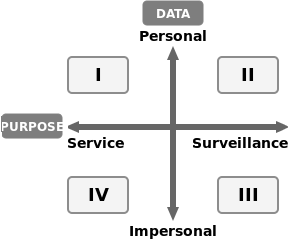
\includegraphics[width=40mm]{images/SmartCityPrivacy}
        \caption{Privacy framework {\parencite[nagemaakt van][]{van2016privacy}}}
        \label{fig:privacy_framework}
    \end{figure}

    In het tweede kwadrant (\textbf{II}) gaat over het verzamelen van data om vervolgens te gebruiken voor monitoren.
    Dit gaat over persoonlijke data die de overheid verzamelt om mensen in de gaten te houden (denk aan politiedata, of beelden van beveiligingscamera’s).
    Het gaat dus om zeer persoonlijke en gevoelige informatie, en mensen ervaren dat ook zo.

    Precies daardoor ligt dit onderwerp onder een vergrootglas.
    Er is veel kritiek op hoe zulke data worden gebruikt voor toezicht en controle.
    Bijvoorbeeld: de burgemeester van Nice kreeg in 2008 een “Big Brother Award” omdat hij de stad vol hing met camera’s.
    Dresden kreeg diezelfde prijs in 2012 voor het volgen van mobiele telefoons tijdens een demonstratie.

    Echter zit hier ook een keerpunt aan, het ligt namelijk aan de huidige tijd en situatie of mensen het een probleem vinden om gemonitord te worden.
    Zo werdt geschreven:
    \qoute{Acceptance of the US government monitoring personal communications was high in the immediate aftermath of the 9/11 attacks but declined after about half a year.}{van2016privacy}{474}
    \\
    \\
    Het derde kwadrant (\textbf{III}) gaat over data die niet direct aan één persoon gekoppeld zijn, maar wél worden gebruikt om gedrag of situaties te controleren.
    Denk aan verkeersstromen of drukte op stations of evenementen.
    Op het eerste gezicht lijkt dat onschuldig, want het gaat niet om individuen, maar om groepen, patronen, cijfers.

    Steden gebruiken zulke “anonieme” data vaak om beleid te maken.
    Rotterdam heeft bijvoorbeeld een systeem waarin allerlei data worden samengevoegd (van politiedata tot economische cijfers) om te zien waar problemen dreigen te ontstaan.
    Zo kan men “risicowijken” aanwijzen of voorspellen waar criminaliteit waarschijnlijk zal oplaaien\footnote{Ookwel predictive policing genoemd}.

    Maar ook hier zit een gevaar, want hoe meer je die datasets koppelt, hoe makkelijker het wordt om tóch individuele mensen te herkennen, dan verandert zogenaamd anonieme data ineens in persoonlijke data.
    Daardoor ontstaat wantrouwen wat kan leiden burgers en organisaties vrezen dat zulke systemen vooroordelen versterken of leiden tot discriminerende controle, zoals in de VS al vaak is gebeurd.

    \subsection{}
    \editorsonly{Type bron: Wat vinden mensen acceptabel qua privacyzorgen ten opzichte van veiligheid en politie; en Amazon's rol hierin.}
    \parencite{shaffer2021applying} In augustus 2019 sloot Ring een samenwerking met de LBPD\footnote{Long Beach Police Department}, waarmee de politie via de app \textit{Neighbors} toegang kreeg tot videobeelden van Ring-deurbellen. Bewoners kunnen via deze app beelden delen van verdachte activiteiten in hun buurt. Officieel is dat volledig vrijwillig, maar in de praktijk voelt het voor velen als een sluiproute naar een samenleving waarin iedereen elkaar in de gaten houdt.

    De reacties op deze samenwerking zijn gemengd.
    Sommigen zien het als een logische stap in het bestrijden van criminaliteit, want het is niet heel anders dan het opvragen van beelden bij winkels of bedrijven.
    Anderen ervaren het juist als een zorgelijke ontwikkeling, als een vorm van burgerlijke surveillance waarbij politie en een (groot) technologiebedrijf samen steeds dieper doordringen in de privésfeer.

    Wat het ongemak versterkt, is dat niet alleen de politie, maar ook Amazon (het moederbedrijf van Ring) toegang heeft tot deze beelden.
    Veel bewoners gaven aan dat ze de politie op zich vertrouwen, maar Amazon veel minder. “Wat doen ze met die data?” is een veelgehoorde vraag.
    De vrees is dat commerciële belangen en veiligheidsdoelen door elkaar gaan lopen.

    Uiteindelijk draait de discussie niet om de camera’s zelf, maar om macht en controle: wie kijkt er mee, en wie bepaalt wat er met die beelden gebeurt?

    \subsection{}
    \editorsonly{Type bron: Technische kant van slimme deurbellen: hoe}

    \subsection{}
    \editorsonly{Type bron: Technische kant van slimme deurbellen: hoe}

    https://www.researchgate.net/profile/Kayiram-Kavitha/publication/350431496_Smart_Surveillance_with_Smart_Doorbell/links/62721544b1ad9f66c89eb53e/Smart-Surveillance-with-Smart-Doorbell.pdf

De toon van dit onderzoek is bijna naïef optimistisch — alsof technologie vanzelf goed is zolang het maar “smart” heet. De auteurs presenteren hun slimme deurbel als een wonder van efficiëntie: een klein IoT-systeem met een sensor die beweging detecteert, een camera die een foto maakt, en een Raspberry Pi die dat beeld meteen naar de cloud of via e-mail doorstuurt. Handig, zeggen ze, want zo hoef je niet 24/7 camera’s terug te kijken. De deurbel ziet iets, stuurt een melding, klaar.


Maar onder dat technische enthousiasme sluimert iets groters. Want waar de onderzoekers spreken over “veiligheid” en “gemak”, hoor je tussen de regels door iets wat ongemakkelijk schuurt: het idee dat elk huis een klein surveillancesysteem moet worden. Alles — van je voordeur tot je telefoon — is onderdeel van een netwerk dat jou observeert, bewaart, en waarschuwt. Alsof veiligheid niet langer iets is wat we \textit{voelen}, maar wat we \textit{berekenen}.


De paper zegt trots dat het systeem “ook privacy biedt”, omdat beelden enkel worden gemaild naar de geregistreerde gebruiker. Maar tegelijk wordt alles naar de cloud gestuurd — alsof dat geen paradox is. Beelden van gezichten, bewegingen, tijdstippen: allemaal opgeslagen, ergens, door iets.


En dat is precies waar het spannend wordt: de grens tussen beveiliging en surveillance vervaagt. Deze slimme deurbel is geen gadget meer, het is een poortwachter die stilletjes data verzamelt over wat er voor jouw deur gebeurt. En die logica — die “slimme” manier van leven — schuift langzaam onze huizen binnen.


Uiteindelijk gaat dit paper dus niet alleen over techniek, maar over vertrouwen. Vertrouwen in een systeem dat kijkt zodat jij niet hoeft te kijken. En de vraag is: hoeveel gemak zijn we bereid te ruilen voor die geruststelling?




    \section{Conclusie}
    Duidelijk antwoord op je onderzoeksvraag.
    Trek de lijn terug naar contextual integrity: veiligheid en privacy staan niet los van elkaar, maar de balans verschuift zodra technologie te veel buiten de intended context gaat. (max 1 pagina)

    \printbibliography

    \balance % balances last-page columns
\end{document}
